% Канонический TikZ-рисунок варианта 29. Править только здесь.
\long\def\figStereoV29{%
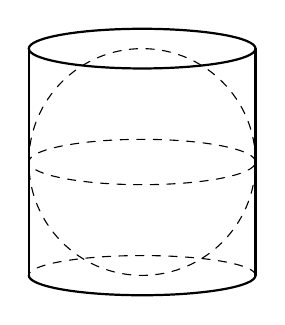
\begin{tikzpicture}[
  scale=0.9,
  line cap=round,
  line join=round
]
  \def\R{1.6}
  \def\H{3.2}
  \def\e{0.28}

  \coordinate (O) at (0,1.6);

  % Шар
  \draw[dashed] (O) circle (\R);
  \draw[dashed]
    (O) ellipse[x radius=\R,y radius=0.32];

  % Верхнее основание цилиндра
  \draw[thick]
    (0,\H) ellipse[x radius=\R,y radius=\e];

  % Образующие цилиндра
  \draw[thick] (-\R,0)--(-\R,\H);
  \draw[thick] ( \R,0)--( \R,\H);

  % Нижнее основание цилиндра
  \draw[thick]
    (-\R,0)
    arc[
      start angle=180,
      end angle=360,
      x radius=\R,
      y radius=\e
    ];

  \draw[dashed]
    (\R,0)
    arc[
      start angle=0,
      end angle=180,
      x radius=\R,
      y radius=\e
    ];
\end{tikzpicture}
}
